% Created 2011-07-17 Sun 09:10
\documentclass{beamer}
\usepackage[utf8]{inputenc}
\usepackage[T1]{fontenc}
\usepackage{fixltx2e}
\usepackage{graphicx}
\usepackage{longtable}
\usepackage{float}
\usepackage{wrapfig}
\usepackage{soul}
\usepackage{textcomp}
\usepackage{marvosym}
\usepackage[integrals]{wasysym}
\usepackage{latexsym}
\usepackage{amssymb}
\usepackage{hyperref}
\tolerance=1000
\usepackage{amsmath}
\usetheme[secheader]{Boadilla}
\usepackage[english]{babel}
\setbeamercolor{title}{fg=black,bg=black!10!brown!50}
\setbeamercolor{block body}{fg=black,bg=black!10!brown!30}
\setbeamercolor{block title}{fg=black,bg=black!30!brown!40}
\setbeamercolor{frametitle}{fg=black,bg=black!30!brown!50}
\beamersetaveragebackground{brown!50!black!20}
\setbeamercolor{author in head/foot}{fg=black,bg=black!30!brown!50}
\setbeamercolor{title in head/foot}{fg=black,bg=black!20!brown!50}
\setbeamercolor{date in head/foot}{fg=black,bg=black!10!brown!50}
\setbeamercolor{section in head/foot}{fg=black,bg=black!30!brown!30}
\setbeamercolor{subsection in head/foot}{fg=black,bg=black!20!brown!30}
\usepackage{animate} %need the animate.sty file 
\usepackage{color}
\usepackage{pgf}
\usepackage{pgfcore}
\usepackage{pgfbaseimage}
\usepackage{pgfbaselayers}
\usepackage{pgfbasepatterns}
\usepackage{pgfbaseplot}
\usepackage{pgfbaseshapes}
\usepackage{pgfbasesnakes}
\usepackage{tikz} 

\tikzset{normal/.style={ 
% The shape: 
rectangle,minimum size=6mm,rounded corners=3mm, 
% The rest 
very thick,draw=black!50, 
top color=white,bottom color=black!20, 
font=\ttfamily}}
\tikzset{arduino/.style={ 
% The shape: 
rectangle, 
% The size: 
minimum size=6mm, 
% The border: 
very thick, 
draw=blue!50!black!50, % 50% red and 50% black, 
% and that mixed with 50% white 
% The filling: 
top color=white, % a shading that is white at the top... 
bottom color=blue!50!black!20, % and something else at the bottom 
% Font 
font=\itshape 
}}
\tikzset{enceinte/.style={ 
% The shape: 
rectangle, 
% The size: 
minimum size=6mm, 
% The border: 
very thick, 
draw=yellow!90!black!50, % 50% red and 50% black, 
% and that mixed with 50% white 
% The filling: 
top color=white, % a shading that is white at the top... 
bottom color=yellow!90!black!20, % and something else at the bottom 
% Font 
font=\itshape 
}}

\tikzset{ordi/.style={ 
% The shape: 
rectangle, 
% The size: 
minimum size=6mm, 
% The border: 
very thick, 
draw=green!90!black!50, % 50% red and 50% black, 
% and that mixed with 50% white 
% The filling: 
top color=white, % a shading that is white at the top... 
bottom color=green!90!black!20, % and something else at the bottom 
% Font 
font=\itshape 
}}

\usetikzlibrary{decorations.pathmorphing,shapes.misc}
\providecommand{\alert}[1]{\textbf{#1}}

\title{Batch, Off-policy and Model-free Apprenticeship Learning}
\author{Edouard Klein and Matthieu Geist and Olivier Pietquin}
\date{\today}

\title[LSTD-$\mu$]{Batch, Off-policy and Model-free Apprenticeship Learning}
\author[Edouard Klein]{\underline{Edouard Klein}$^{\dag\ddag}$, Matthieu Geist$^\dag$ and Olivier Pietquin$^\dag$\\\texttt{firstname.lastname@supelec.fr}\\\url{http://www.metz.supelec.fr/metz/personnel/klein_edo/ALIHT2011.pdf}}\institute[Supélec]{$\dag$Supélec UMI 2958 (GeorgiaTech - CNRS), France\\$\ddag$Equipe ABC UMR 7503 (LORIA-CNRS), France}
\begin{document}

\maketitle











\tikzstyle{state}=[circle,
thick,
minimum size=1.0cm,
draw=blue!80,
fill=blue!20]
\tikzstyle{action}=[rectangle,thick,
minimum size=1.0cm,
draw=orange!80,
fill=orange!20]
\tikzstyle{element}=[rectangle,
thick,
minimum size=1.0cm,
draw=blue!80,
fill=blue!20]
\tikzstyle{action}=[rectangle,thick,
minimum size=1.0cm,
draw=orange!80,
fill=orange!20]
\section{Non-technical Abstract}
\label{sec-1}
\subsection{Context}
\label{sec-1_1}
\begin{frame}
\frametitle{Reinforcement Learning}
\label{sec-1_1_1}
\begin{columns}
\begin{column}{0.4\textwidth}
%% Toto
\label{sec-1_1_1_1}

     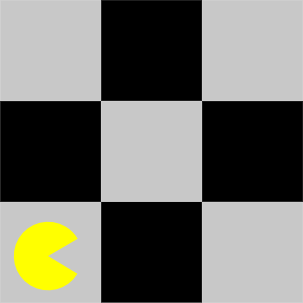
\includegraphics[width=10em]{ML.png}
\end{column}
\begin{column}{0.4\textwidth}
\begin{block}{Notions}
\label{sec-1_1_1_2}


\begin{itemize}
\item Agent
\item Task
\item Environment
\end{itemize}
\end{block}
\end{column}
\end{columns}
\end{frame}
\begin{frame}
\frametitle{Imitation: Expert}
\label{sec-1_1_2}

     \animategraphics[autoplay,loop,height=5cm]{1}{Expert00}{1}{9} 
\end{frame}
\begin{frame}
\frametitle{Imitation: Generalization}
\label{sec-1_1_3}
\begin{columns}
\begin{column}{.4\textwidth}
%% Null
\label{sec-1_1_3_1}

      \animategraphics[autoplay,loop,height=5cm]{1}{Agent}{001}{014} 
\end{column}
\begin{column}{.4\textwidth}
\begin{block}{Apprenticeship learning}
\label{sec-1_1_3_2}

     Reward inference
\end{block}
\end{column}
\end{columns}
\end{frame}
\subsection{Contribution}
\label{sec-1_2}
\begin{frame}
\frametitle{Contribution}
\label{sec-1_2_1}

\uncover<1->{
  \begin{block}{Abbeel and Ng's IRL}
    \label{sec-1_2_1_1}

    \begin{tikzpicture}
      \node[element] (trajE) at (0,0) {$\vcenter{\hbox{
\includegraphics[height=0.5cm]{Expert.png}}}$Trajectories} ;
      \node[action] (mech) at (3,-0.7) {
\includegraphics[height=0.5cm]{Moulinette.png}} ;
      \node[element] (policy) at (5,-0.7) {$\vcenter{\hbox{
\includegraphics[height=0.5cm]{Pi.png}}}$Policy} ;
      \node[action] (sim) at (8,-0.7) {$\vcenter{\hbox{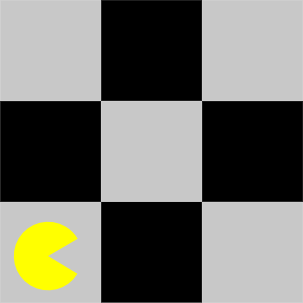
\includegraphics[height=0.5cm]{ML.png}}}$Simulator} ;
      \node[element] (trajA) at (0,-1.4) {$\vcenter{\hbox{
\includegraphics[height=0.5cm]{Agent.png}}}$Trajectories} ;
      \draw [->,thick] (trajE.east) .. controls (2,0) and (2,-0.7) .. (mech.west);
      \draw [->,thick] (trajA.east) .. controls (2,-1.4) and (2,-0.7) .. (mech.west);  
      \draw [->,thick] (mech.east) -- (policy.west);
      \draw [->,thick] (policy.east) -- (sim.west);
      \draw [->,thick] (sim.east) -- (10,-0.7) -- (10,-2.1) -- (0,-2.1) -- (trajA.south);
    \end{tikzpicture}
  \end{block}
}
\uncover<2->{
\begin{block}{LSTD-$\mu$}
\label{sec-1_2_1_2}

  \begin{tikzpicture}
    \node[element] (trajE) at (0,0) {$\vcenter{\hbox{
\includegraphics[height=0.5cm]{Expert.png}}}$Transitions} ;
    \node[action] (mech) at (3,-0.7) {
\includegraphics[height=0.5cm]{Moulinette.png}} ;
    \node[element] (policy) at (5,-0.7) {$\vcenter{\hbox{
\includegraphics[height=0.5cm]{Pi.png}}}$Policy} ;
    \node[element] (trajA) at (0,-1.4) {$\vcenter{\hbox{
\includegraphics[height=0.5cm]{Agent.png}}}$Transitions} ;
    \draw [->,thick] (trajE.east) .. controls (2,0) and (2,-0.7) .. (mech.west);
    \draw [->,thick] (trajA.east) .. controls (2,-1.4) and (2,-0.7) .. (mech.west);  
    \draw [->,thick] (mech.east) -- (policy.west);
    \draw [->,thick] (policy.east) -- (10,-0.7) -- (10,-1.4) -- (3,-1.4) -- (mech.south);
  \end{tikzpicture}
\end{block}
}
\end{frame}
\section{IRL}
\label{sec-2}
\subsection{RL}
\label{sec-2_1}
\begin{frame}
\frametitle{Quick definitions}
\label{sec-2_1_1}

       \begin{columns}
    \begin{column}{4cm}
      \begin{block}{}
        \begin{overlayarea}{\textwidth}{4.4cm}
          \only<1>{\begin{tikzpicture}
  \node[state] (st) at (0,0) {$s_t$};
  \node at (0,1.5) {};
\end{tikzpicture}
}
          \only<2>{\begin{tikzpicture}
  \node[state] (st) at (0,0) {$s_t$};
  \node[action] (st) at (1.5,-2) {$a_{t}$};
  \node at (0,1.5) {};
\end{tikzpicture}
}
          \only<3>{\begin{tikzpicture}
  \node[state] (st) at (0,0) {$s_t$};
  \node[action] (at) at (1.5,-2) {$a_{t}$};
  \node[state] (stpu) at (3,0) {$s_{t+1}$};
  \draw[->,thick] (at) --  (stpu);
  \draw[->,thick] (st) -- node[below] {$p(s_{t+1}|s_t,a_t)$}(stpu);
  \node at (0,1.5) {};
\end{tikzpicture}
}
          \only<4->{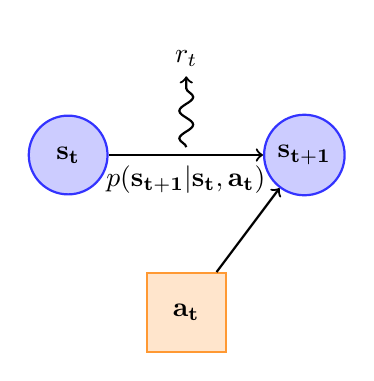
\begin{tikzpicture}
\tikzstyle{state}=[circle,
thick,
minimum size=1.0cm,
draw=blue!80,
fill=blue!20]
\tikzstyle{action}=[rectangle,thick,
minimum size=1.0cm,
draw=orange!80,
fill=orange!20]

  \node[state] (st) at (0,0) {$\mathbf{s_t}$};
  \node[action] (at) at (1.5,-2) {$\mathbf{a_{t}}$};
  \node[state] (stpu) at (3,0) {$\mathbf{s_{t+1}}$};
  \draw[->,thick] (at) --  (stpu);
  \draw[->,thick] (st) -- node[below] {$p(\mathbf{s_{t+1}}|\mathbf{s_t},\mathbf{a_t})$}(stpu);
  \draw[->,thick,decorate,decoration={snake}] (1.5,0.1) -- (1.5,1);
  \node[anchor=south] at (1.5,1.0) {$r_t$};
  \node at (0,1.5) {};
\end{tikzpicture}
}
        \end{overlayarea}
      \end{block}
    \end{column}
    \begin{column}{4cm}
      \begin{block}{Notions}
        \begin{itemize}
          \item<1-> State $s_t\in S$
          \item<2-> Action $a_t \in A$
          \item<3-> Reward $r_t \in \mathbb{R}$
          \item<4-> Transition $(s_t,a_t,s_{t+1},r_t)\in S\times A\times S\times\mathbb{R}$
        \end{itemize}
      \end{block}
      \begin{block}<1->{Markovian criterion}
        Past states are irrelevant
      \end{block}
    \end{column}
  \end{columns}
  \begin{alertblock}<5>{Policy}
    $\pi: S\rightarrow A$
  \end{alertblock}
\end{frame}
\begin{frame}
\frametitle{RL problem and solution}
\label{sec-2_1_2}
\begin{block}<1->{Value function}
\label{sec-2_1_2_1}

     \begin{equation}
     \label{eqn:V}
     V^\pi(s_t) = E\left[\left.\sum\limits_{i}\gamma^i r_{t+i}\right|\pi\right]
     \end{equation}
\end{block}
\begin{block}<2->{Goal}
\label{sec-2_1_2_2}

     Optimal policy $\pi^* = \arg\max\limits_\pi V^\pi$
\end{block}
\begin{block}<3->{Value function approximation}
\label{sec-2_1_2_3}

     $\hat V^\pi(s_t) = \omega^T\phi (s_t)$
\end{block}
\end{frame}
\subsection{IRL}
\label{sec-2_2}
\begin{frame}
\frametitle{IRL problem and solutions}
\label{sec-2_2_1}
\begin{block}<1->{Goal}
\label{sec-2_2_1_1}

     Finding the reward $R$ so that the observed behavior is optimal
\end{block}
\begin{alertblock}<2->{Ill-posed}
\label{sec-2_2_1_2}

     The null reward $\forall s, R(s) = 0$ is a solution
\end{alertblock}
\begin{block}<3->{Approximation of the reward}
\label{sec-2_2_1_3}

     $R = \theta^T\phi(s)$
\end{block}
\end{frame}
\begin{frame}
\frametitle{IRL solutions}
\label{sec-2_2_2}
\begin{block}{Introduction of the expected, cumulative, discounted feature values}
\label{sec-2_2_2_1}

     \scriptsize
     \begin{eqnarray*}
     V^\pi(s_t) &=& E\left[\left.\sum\limits_{i}\gamma^i r_{t+i}\right|\pi\right]\\
     V^\pi(s_t) &=& E\left[\left.\sum\limits_{i}\gamma^i \theta^T\phi(s_{t+i})\right|\pi\right]\\
     V^\pi(s_t) &=& \theta^T\underbrace{E\left[\left.\sum\limits_{i}\gamma^i \phi(s_{t+i})\right|\pi\right]}_{\mu^\pi(s_t)}\\
     V^\pi(s_t) &=& \theta^T\mu^\pi(s_t)
     \end{eqnarray*}
\end{block}
\end{frame}
\begin{frame}
\frametitle{IRL solutions}
\label{sec-2_2_3}
\begin{block}{Importance of $\Delta\mu$}
\label{sec-2_2_3_1}

     \begin{eqnarray*}
     \Delta\mu &=& ||\mu_E(s_0) - \mu^\pi(s_0)||_2\\
     \Delta V &=& |V^E(s_0) - V^\pi(s_0)|\\
     \Delta V &=& |\theta^T\left(\mu_E(s_0) - \mu^\pi(s_0)\right)|\\
     \Delta V &\leq& ||\theta||_2||\mu_E(s_0) - \mu^\pi(s_0)||_2\\
     \Delta V &\leq& \Delta\mu\\
     \end{eqnarray*}
\end{block}
\end{frame}
\begin{frame}
\frametitle{Computing $\mu$}
\label{sec-2_2_4}
\begin{columns}
\begin{column}{.4\textwidth}
\begin{block}<1->{Monte carlo}
\label{sec-2_2_4_1}

     $\hat\mu^\pi(s_0) = \sum\limits_j\sum\limits_i\gamma^i\phi(s^j_i)$
\end{block}
\begin{block}<1->{Drawbacks}
\label{sec-2_2_4_2}


\begin{itemize}
\item Needs whole trajectories
\item Implies using a simulator
\begin{itemize}
\item Need for a model
\item On-policy evaluation
\end{itemize}
\end{itemize}
\end{block}
\end{column}
\begin{column}{.4\textwidth}
\begin{block}<2->{LSTD-$\mu$}
\label{sec-2_2_4_3}

     Based on already known \emph{Least-square temporal differences} method
\end{block}
\begin{block}<2->{Advantages}
\label{sec-2_2_4_4}


\begin{itemize}
\item Can be fed with transitions
\item No simulator needed
\begin{itemize}
\item No need for a model
\item Off or on policy evaluation
\end{itemize}
\end{itemize}
\end{block}
\end{column}
\end{columns}
\end{frame}
\section{LSTD-$\mu$}
\label{sec-3}
\subsection{LSTD \& LSTDQ}
\label{sec-3_1}
\begin{frame}
\frametitle{LSTD algorithms}
\label{sec-3_1_1}
\begin{block}<1->{LSTD and LSTD-$Q$}
\label{sec-3_1_1_1}

     Batch, off or on-policy, model-free \emph{state} or \emph{state-action} \emph{value function approximation} algorithm
\end{block}
\begin{block}<2->{Principle}
\label{sec-3_1_1_2}

     Estimator : $\hat V^\pi(s) = \omega^T\phi(s)$ \hfill Transition: $s_t,a_t,s_{t+1},r_t$
     \begin{equation*}
     \omega = \left(\sum_{t=1}^n
     \phi(s_t)(\phi(s_t)-\gamma\phi(s_{t+1}))^T\right)^{-1}
     \sum_{t=1}^n \phi(s_t) r_t
     \end{equation*}
     \begin{equation*}
     \omega = LSTD_\phi( \{s_t,a_t,s_{t+1}\}_t,\{{ r_t}\}_t)
     \end{equation*}
\end{block}
\end{frame}
\subsection{LSTD-$\mu$}
\label{sec-3_2}
\begin{frame}
\frametitle{LSTD-$\mu$ algorithm}
\label{sec-3_2_1}
\begin{block}<1->{Idea}
\label{sec-3_2_1_1}

     $V = V^\pi(s_t) = E\left[\left.\sum\limits_{i}\gamma^i r_{t+i}\right|\pi\right]$
     \hfill $\mu^\pi(s_t) = E\left[\left.\sum\limits_i\gamma^i\phi(s_{t+i})\right|\pi\right]$ \\
     \begin{center}
     Transition: $s_t,a_t,s_{t+1},r_t$
     \end{center}
\end{block}
\begin{columns}
\begin{column}{.45\textwidth}
\begin{block}<2->{LSTD}
\label{sec-3_2_1_2}

     Estimator : $\hat V^\pi(s) = \omega^T\phi(s)$
     \begin{equation*}
     \omega = LSTD_{\color{red}\phi}( \{s_t,a_t,s_{t+1}\}_t,\{{\color{red}r_t}\}_t)
     \end{equation*}
\end{block}
\end{column}
\begin{column}{.5\textwidth}
\begin{block}<2->{LSTD-$\mu$}
\label{sec-3_2_1_3}

     Estimator : $\hat \mu^\pi(s) = \xi^{T}\psi(s)$
     \begin{equation*}
     \xi_i = LSTD_{\color{red}\psi}( \{s_t,a_t,s_{t+1}\}_t, \{{\color{red}\phi_i(s_t)}\}_t )
     \end{equation*}
\end{block}
\end{column}
\end{columns}
\end{frame}
\section{Experimental benchmark}
\label{sec-4}
\subsection{Algorithms}
\label{sec-4_1}
\begin{frame}
\frametitle{Algorithms: Abbeel \& Ng's IRL algorithm}
\label{sec-4_1_1}
\begin{block}{Principle}
\label{sec-4_1_1_1}

     \begin{tikzpicture}
     \node[element] (trajE) at (0,0) {$\vcenter{\hbox{
\includegraphics[height=0.5cm]{Expert.png}}}$Trajectories} ;
     \node[action] (mech) at (3,-0.7) {
\includegraphics[height=0.5cm]{Moulinette.png}} ;
     \node[element] (policy) at (5,-0.7) {$\vcenter{\hbox{
\includegraphics[height=0.5cm]{Pi.png}}}$Policy} ;
     \node[action] (sim) at (8,-0.7) {$\vcenter{\hbox{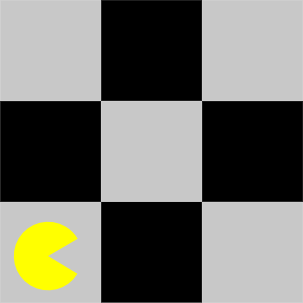
\includegraphics[height=0.5cm]{ML.png}}}$Simulator} ;
     \node[element] (trajA) at (0,-1.4) {$\vcenter{\hbox{
\includegraphics[height=0.5cm]{Agent.png}}}$Trajectories} ;
     \draw [->,thick] (trajE.east) .. controls (2,0) and (2,-0.7) .. (mech.west);
     \draw [->,thick] (trajA.east) .. controls (2,-1.4) and (2,-0.7) .. (mech.west);  
     \draw [->,thick] (mech.east) -- (policy.west);
     \draw [->,thick] (policy.east) -- (sim.west);
     \draw [->,thick] (sim.east) -- (10,-0.7) -- (10,-2.1) -- (0,-2.1) -- (trajA.south);
     \end{tikzpicture}
\end{block}
\begin{columns}
\begin{column}{.45\textwidth}
\begin{block}{Variants}
\label{sec-4_1_1_2}


\begin{itemize}
\item Monte-Carlo estimation
\item Projection method
\item LSPI as the MDP solver
\end{itemize}
\end{block}
\end{column}
\begin{column}{.45\textwidth}
\begin{block}{Update step}
\label{sec-4_1_1_3}

     $t = \max\limits_{\theta}\min\limits_{\pi}\theta^T(\mu^{E}(s_0)-\mu^{\pi}(s_0))$
\end{block}
\end{column}
\end{columns}
\end{frame}
\begin{frame}
\frametitle{Algorithms: Our modified version}
\label{sec-4_1_2}
\begin{block}{Principle}
\label{sec-4_1_2_1}

     \begin{tikzpicture}
     \node[element] (trajE) at (0,0) {$\vcenter{\hbox{
\includegraphics[height=0.5cm]{Expert.png}}}$Transitions} ;
     \node[action] (mech) at (3,-0.7) {
\includegraphics[height=0.5cm]{Moulinette.png}} ;
     \node[element] (policy) at (5,-0.7) {$\vcenter{\hbox{
\includegraphics[height=0.5cm]{Pi.png}}}$Policy} ;
     \node[element] (trajA) at (0,-1.4) {$\vcenter{\hbox{
\includegraphics[height=0.5cm]{Agent.png}}}$Transitions} ;
     \draw [->,thick] (trajE.east) .. controls (2,0) and (2,-0.7) .. (mech.west);
     \draw [->,thick] (trajA.east) .. controls (2,-1.4) and (2,-0.7) .. (mech.west);  
     \draw [->,thick] (mech.east) -- (policy.west);
     \draw [->,thick] (policy.east) -- (10,-0.7) -- (10,-1.4) -- (3,-1.4) -- (mech.south);
     \end{tikzpicture}
\end{block}
\begin{columns}
\begin{column}{.45\textwidth}
\begin{block}{Variants}
\label{sec-4_1_2_2}


\begin{itemize}
\item \emph{LSTD-$\mu$ estimation}
\item Projection method
\item LSPI as the MDP solver
\end{itemize}
\end{block}
\end{column}
\begin{column}{.45\textwidth}
\begin{block}{Update step}
\label{sec-4_1_2_3}

     $t = \max\limits_{\theta}\min\limits_{\pi}\theta^T(\mu^{E}(s_0)-\mu^{\pi}(s_0))$
\end{block}
\end{column}
\end{columns}
\end{frame}
\subsection{Quality criterion}
\label{sec-4_2}
\begin{frame}
\frametitle{Quality criterion}
\label{sec-4_2_1}

\center
\resizebox{.9\columnwidth}{!}{\input{../CodeJFPDA/GridWorld/criteria_mc}}
\end{frame}
\subsection{GirdWorld}
\label{sec-4_3}
\begin{frame}
\frametitle{Settings}
\label{sec-4_3_1}
\begin{columns}
\begin{column}{0.4\textwidth}
%% Toto
\label{sec-4_3_1_1}

     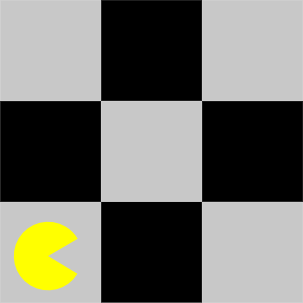
\includegraphics[width=10em]{ML.png}
\end{column}
\begin{column}{0.4\textwidth}
\begin{block}{Mathematically}
\label{sec-4_3_1_2}

     

\begin{itemize}
\item $A = \{$ Up, Down, Right, Left $\}$
\item $S = {cells}$
\item $\phi$: discrete features
\item Reward in the upper right corner
\end{itemize}
\end{block}
\end{column}
\end{columns}
\end{frame}
\begin{frame}
\frametitle{Results}
\label{sec-4_3_2}

\center
\resizebox{.9\columnwidth}{!}{\input{../CodeJFPDA/GridWorld/both_error_EB}}
\end{frame}
\subsection{Inverted pendulum}
\label{sec-4_4}
\begin{frame}
\frametitle{Settings}
\label{sec-4_4_1}
\begin{columns}
\begin{column}{0.4\textwidth}
%% Toto
\label{sec-4_4_1_1}

     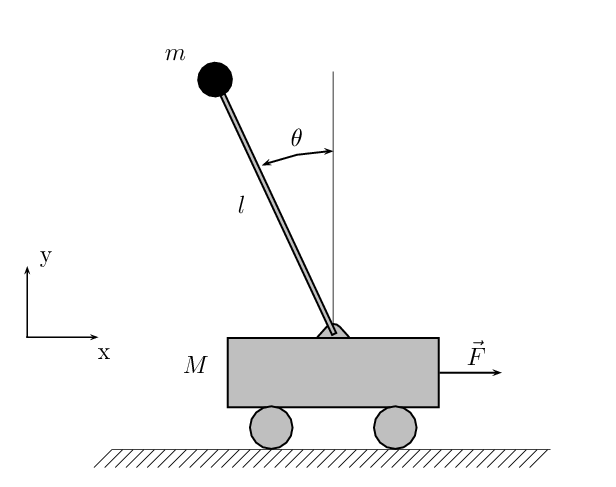
\includegraphics[width=10em]{InvertedPendulum.png}
\end{column}
\begin{column}{0.55\textwidth}
\begin{block}{Mathematically}
\label{sec-4_4_1_2}


\begin{itemize}
\item $A = \{$ Left, Nothing, Right $\}$
\item $S = {speed,angle}$
\item $\phi$: Gaussian network and a constant
\item Negative reward for letting it fall
\end{itemize}
\end{block}
\end{column}
\end{columns}
\end{frame}
\begin{frame}
\frametitle{Results (one run)}
\label{sec-4_4_2}

\center
\resizebox{.9\columnwidth}{!}{\input{../CodeJFPDA/InvertedPendulum/threshold}}
\end{frame}
\begin{frame}
\frametitle{Results (average)}
\label{sec-4_4_3}

\center
\resizebox{.9\columnwidth}{!}{\input{../CodeJFPDA/InvertedPendulum/threshold_EB}}
\end{frame}
\section{Opening and future work}
\label{sec-5}
\subsection{Future work}
\label{sec-5_1}
\begin{frame}
\frametitle{Possible future work}
\label{sec-5_1_1}
\begin{itemize}

\item Other $\mu$ based algorithms\\
\label{sec-5_1_1_1}%
\item New tests on harder problems\\
\label{sec-5_1_1_2}%
\item Transferring the reward, and not the policy\\
\label{sec-5_1_1_3}%
\end{itemize} % ends low level
\end{frame}
\begin{frame}
\frametitle{Thank you\ldots{}}
\label{sec-5_1_2}

    \ldots{} for your attention
\end{frame}

\end{document}
